%==============================================================================
%== template for LATEX poster =================================================
%==============================================================================
%
%--A0 beamer slide-------------------------------------------------------------
\documentclass[final]{beamer}
\usepackage[orientation=portrait,size=a0,
            scale=1.25         % font scale factor
           ]{beamerposter}

\geometry{
  hmargin=2.5cm, % little modification of margins
}

%
\usepackage[utf8]{inputenc}
\usepackage{pgfplots}

\linespread{1.15}

\begin{filecontents}{sub_mnn.csv}
submission,score
1,0.166
2,0.232
3,0.305
4,0.348
5,0.481
6,0.518
7,0.528
8,0.564
\end{filecontents}


\begin{filecontents}{sub_cnn.csv}
submission,score
9,0.532
10,0.100
11,0.106
12,0.848
\end{filecontents}

%
%==The poster style============================================================
\usetheme{sharelatex}

%==Title, date and authors of the poster=======================================
\title
%[Super Conference, 1 - 10 July 2013, New York, USA] % Conference
[Final Presentation for ML Course, June 13th 2017, Beijing]
{ % Poster title
Freesound General-Purpose Audio Tagging Challenge
}

\author{ % Authors
Usama Zafar, Sarah Gross
}
\institute
{
	Tsinghua University, China
}
\date{\today}



\begin{document}
\begin{frame}[t]
%==============================================================================
\begin{multicols}{3}
%==============================================================================
%==The poster content==========================================================
%==============================================================================

\section{Introduction}

	Sound surrounds us. Some are distinct and instantly recognizable, like a baby's laugh or the strum of a guitar. Other sounds aren't clear and are difficult to pinpoint, or are drowned in a mix of sounds that are difficult to identify individually.\\

	\begin{figure}
	\centering
	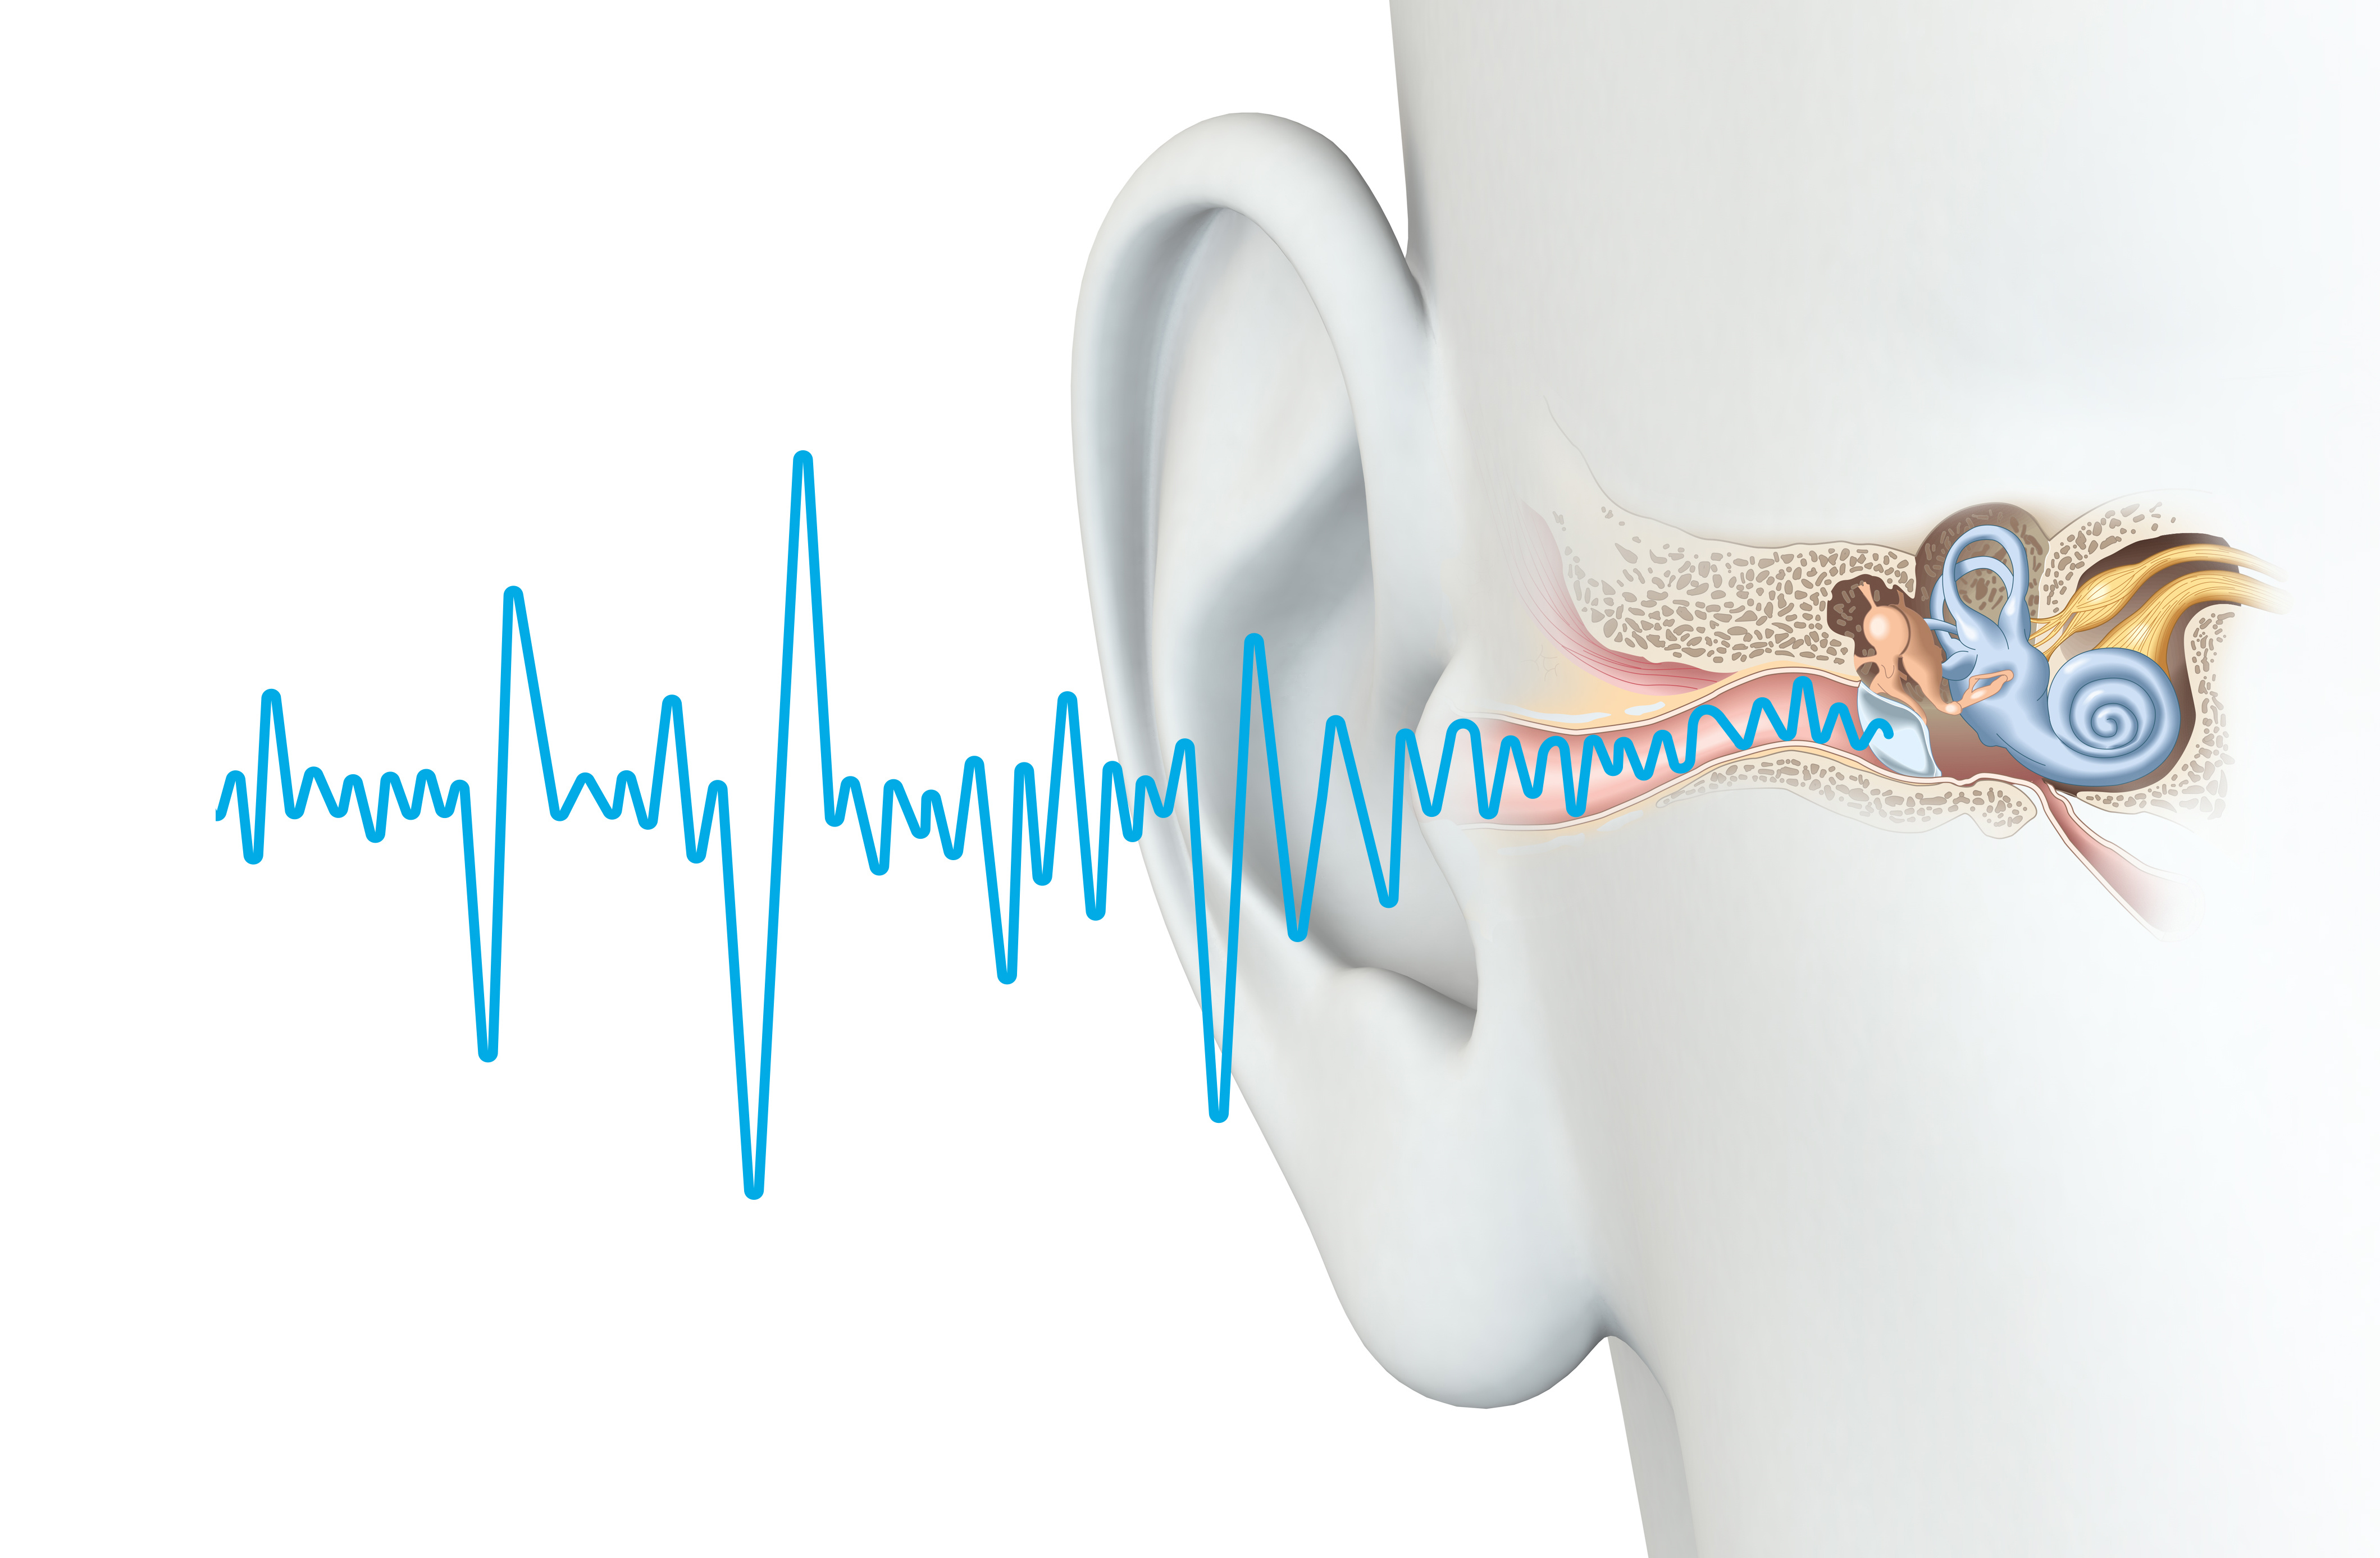
\includegraphics[width=0.4\columnwidth]{ear_sound.jpg}
	\end{figure}

	A lot of research has been done for speech recognition, but little tackle the issue of recognizing environmental sounds. Yet, it can have many applications, from automatic deaf-annotation on videos to robotics.\\
	This project's goal is to be able to classify successfully sound events of very diverse natures.

\section{Background}

	Earlier works \cite{ref1} \cite{ref2} created algorithms based on Hidden Markov Models for this task, as this technique proved very efficient for speech recognition.\\
	However many other authors \cite{ref3} \cite{ref4} disapproved this approach, as environmental sound is not structured data following a logical path like speech, making HMM unreliable.\\
	Toyoda et. al. \cite{ref5} show that Neural Networks give similar results on general sound classification than HMM for less computation, and most recently research on Convolutional Neural Networks \cite{ref4} \cite{ref6} gave noise-independant, excellent results for this task (92,19\% accuracy for CNN vs 57.4\% accuracy for HMM \cite{ref4}).

\section{Method}

	\subsection{Feature extraction}

		Raw waves contain too much unecessary information, thus feature extraction process can reduce the size of data, remove redundancy or background noise, \dots \\

		The most important feature are Mel Frequency Cepstral Coefficents (MFCCs). They are widely used in speech recognition, and give valuable information about the audio file. They are in log scale, which simulates the way the human ear perceives sounds.\\

		\begin{figure}
		\centering
		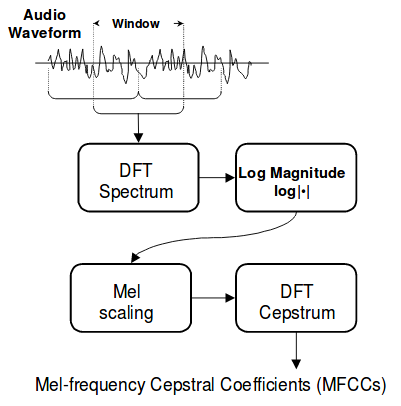
\includegraphics[width=0.8\columnwidth]{steps_mfcc.png}
		\caption{Flowchart for MFCC computation}
		\end{figure}

		We use python library \textit{LibROSA} for feature extraction. On top of MFCC, we extract \textit{chroma, mel, contrast, tonnetz}, which are other useful sound features. Parallelization of code using threads was implemented, dividing by 4 the running time. Extraction step being by far the longest, features are stored in files in order to run several times classification without needing to extract them again.

		\vskip1ex
		\begin{figure}
		\centering
		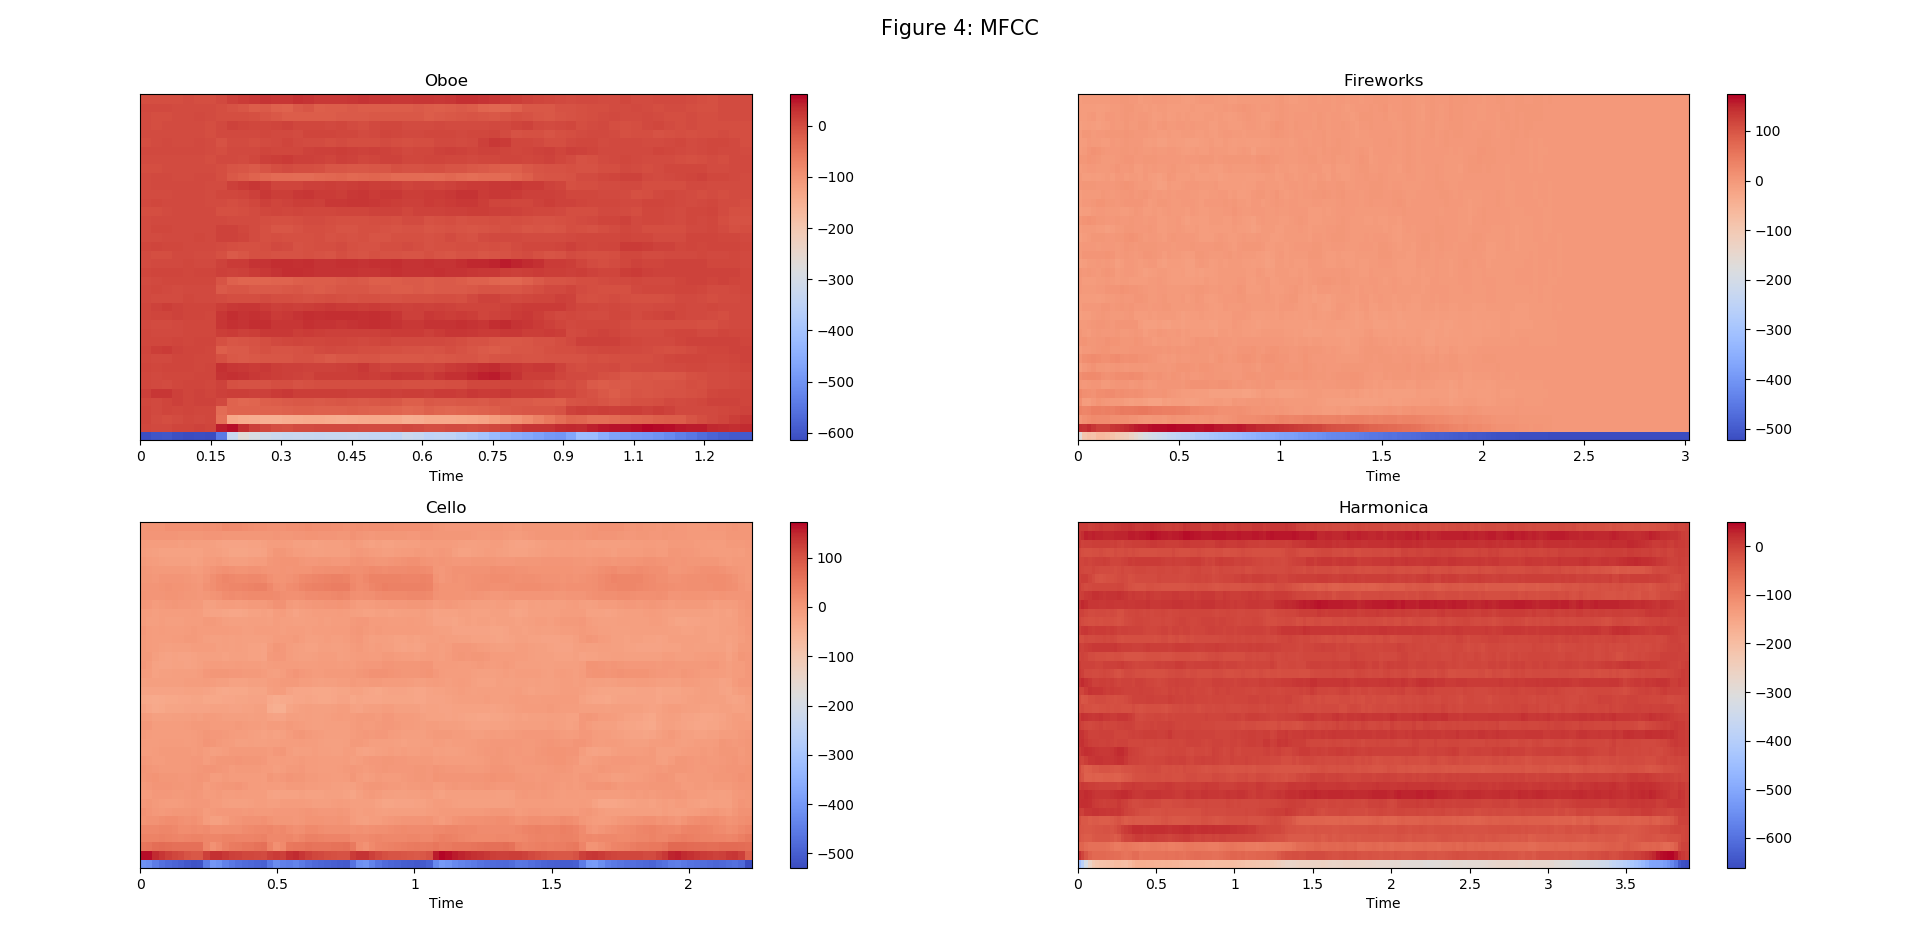
\includegraphics[width=0.99\columnwidth]{mfcc.png}
		\caption{MFCCs on some example sounds}
		\end{figure}
		\vskip2ex
		

	\subsection{Classification}

		After extracting the features, they are fed to a multilayer neural network.

		\vskip2ex
		\begin{table}
		\centering
		\caption{Tensorflow MNN settings}
		\begin{tabular}{ccccc}
		\hline\hline
		Parameter & Chosen value\\
		\hline
		Number layers & 3\\
		Neurons per layer & 200, 250, 300\\
		Act func per layer & tanh, sig, sig\\
		Learning rate & 0.005 (exp decay)\\
		Cost function & cross entropy\\
		Optimize & adam\\ 
		Num epochs & 500\\
		\hline\hline
		\end{tabular}
		\end{table}
		\vskip2ex

		These settings were obtained by try-and-fail run of code, and checking the cost graph.\\

		After MNN, we implemented a 2D-CNN in order to compare and combine the techniques.\\
		We divide each sound clip into 40x173 segments and use only MFCC feature as channel.

		\vskip1ex
		\begin{figure}
		\centering
		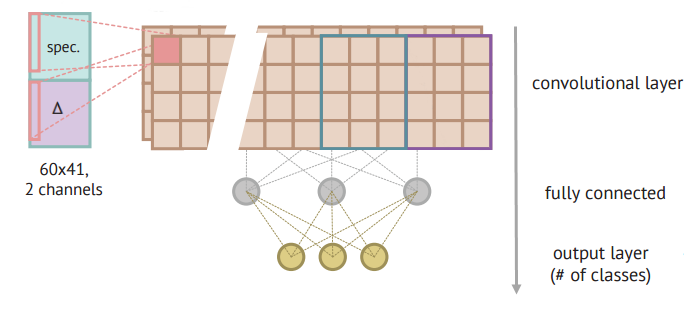
\includegraphics[width=0.99\columnwidth]{cnn_chart.png}
		\caption{Schema of implemented CNN}
		\end{figure}
		\vskip2ex

		We first tried to use Tensorflow, then switched to an easier implementation with Keras with 4 convolutional layers, "same" padding and ReLu activation functions.


\section{Experiments and results}

	\subsection{Evaluation}
		The code was tested on Freesound Kaggle Dataset 2018, containing 18,873 .wav files annotated with 41 labels from Google's AudioSet Ontology.\\

		For each sound file, we give 3 most likely labels.
		Submissions are evaluated according to the Mean Average Precision @ 3 (MAP@3):

		$$MAP@3 = \frac{1}{U} \displaystyle\sum_{u=1}^U \displaystyle\sum_{k=1}^{3}P(k)$$\\

		where $U$ is the number of scored audio files in the test data, $P(k)$ is the precision at cutoff k.


	\subsection{Results}
		Left: our MAP@3 score progression curve. Right: The MNN cross-entropy loss graph.
		\begin{center}
		\begin{minipage}{.59\linewidth}
		\begin{tikzpicture}
		\tikzstyle{every node}=[font=\small]
		\centering
            \begin{axis}[width=0.90\columnwidth, height=250, ylabel=Score, xlabel=Submission, ytick={0.1,0.2,0.3,0.4,0.5,0.6,0.7,0.8,0.9}, xtick={0,2,4,6,8,10,12},xlabel style={yshift=-0.5cm}, ylabel style={yshift=1cm}, legend pos=north west]
                \addplot[thick, blue] table [x=submission, y=score, col sep=comma ] {sub_mnn.csv};
                \addlegendentry{MNN}
                \addplot[thick, red!70!yellow] table [x=submission, y=score, col sep=comma ] {sub_cnn.csv};
                \addlegendentry{CNN}
            \end{axis}
        \end{tikzpicture}
        \end{minipage}
		\begin{minipage}{.39\linewidth}
		\begin{tikzpicture}
		\tikzstyle{every node}=[font=\small]
		\centering
            \begin{axis}[width=0.90\columnwidth, height=250, ylabel=Cost, xlabel=Num of epochs,xtick={0,200,400,600}, ytick={0,1000,2000,3000,4000}, xlabel style={yshift=-0.5cm}, ylabel style={yshift=1.7cm}]
                \addplot[thick, blue] table [x=epoch, y=cost, col sep=comma, ] {cost_history_mnn.csv};
            \end{axis}
        \end{tikzpicture}
        \end{minipage}
        \end{center}
        \vskip2ex


        We built the MNN confusion matrix for the 10 most frequent labels. The model makes less mistakes on the musical instruments than on the other sounds.
		\begin{figure}
		\centering
		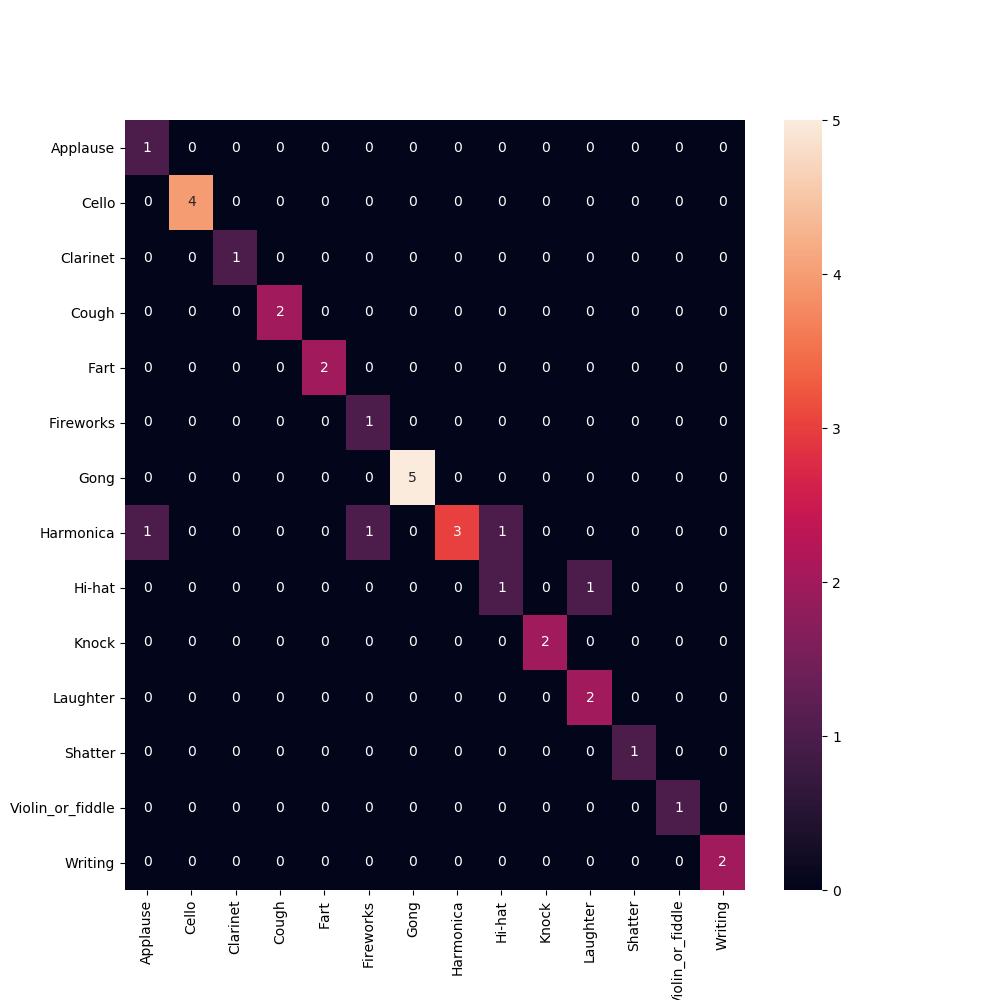
\includegraphics[width=0.90\columnwidth]{confusion_matrix.png}
		\caption{Confusion Matrix (x: prediction, y: true label)}
		\end{figure}

\section{Conclusion}

	This work presents a classification method of environmental sounds based on neural networks. We get an algoritmn running feature extraction within an hour and classification in a few minutes. It classifies correctly 56,4\% of the data with MNN and 84,8\% of the data using 2D-CNN, which is consistent with the results in the literature \cite{ref4} \cite{ref5} \cite{ref6}.
	In order to further improve our model, we could combine their results and add a 1D-CNN.


%==============================================================================
%==End of content==============================================================
%==============================================================================
\subsection{Acknowledgments}
	We are grateful to Tsinghua University's Department of Computer Science for providing us the ressources necessary for this project,
	and to Prof. Zhu and Tang for their guidance.

%--References------------------------------------------------------------------

\subsection{References}

\begin{thebibliography}{99}

\bibitem{ref1} A. Dufaux, L. Besacier, M. Ansorge, and F. Pellandini, Automatic sound de-
tection and recognition for noisy environment. In \textit{IEEE 10th European Signal Processing Conference}, 2000.

\bibitem{ref2} M. Casey, General sound classification and similarity in mpeg-7. In \textit{Organised Sound},volume 6, 2001.

\bibitem{ref3} M. Cowling and R. Sitte, Comparison of techniques for environmental sound recognition. In \textit{Elsevier, Pattern Recognition Letters}, volume 24, 2003.

\bibitem{ref4} H. Zhang, I. McLoughlin, and Y. Song., Robust sound event recognition using convolutional neural networks. In \textit{IEEE International Conference on Acoustics, 
Speech and Signal Processing (ICASSP)}, 2015.

\bibitem{ref5} Y. Toyoda, J. Huang, S. Ding and Y. Liu, "Environmental sound recognition by multilayered neural networks," \textit{CIT '04. The Fourth International Conference on computer and Information Technology}, 2004, pp. 123-127.

\bibitem{ref6} K. Piczak. Environmental sound classification with convolutional neural networks. In\textit{IEEE international workshop on Machine Learning for signal processing}, 2015.

\end{thebibliography}
%--End of references-----------------------------------------------------------

\end{multicols}

%==============================================================================
\end{frame}
\end{document}
